\documentclass[standalone, version=1.0]{huangfusl-template}
\usepackage{amsmath}
\usepackage{tikz}
\usepackage{pgfplots}
\begin{document}
    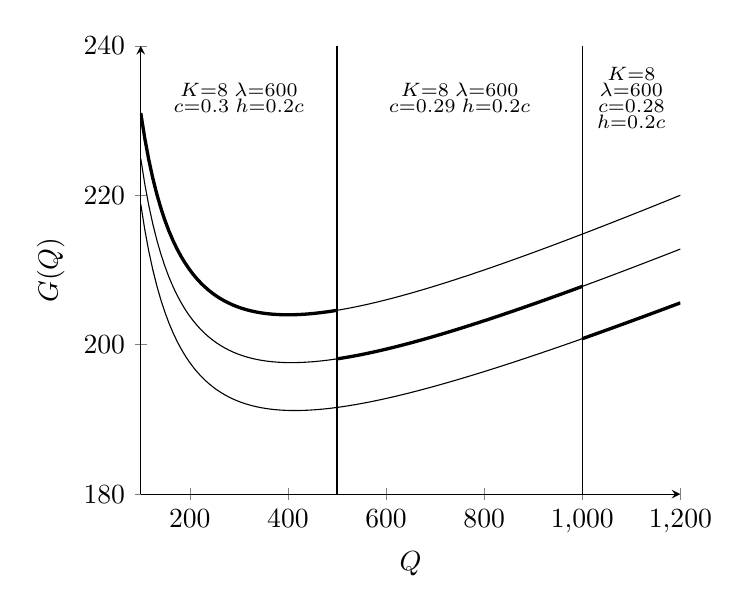
\begin{tikzpicture}
        \begin{axis}[
            axis lines = left,
            ymin=180,
            ymax=240,
            restrict y to domain=180:240,
            xmin=100,
            xmax=1200,
            restrict x to domain=100:1200,
            xlabel = $Q$,
            ylabel = {$G(Q)$},
        ]
            \addplot[domain=100:500, samples=50, very thick] {4800 / x + 180 + 0.03 * x};
            \addplot[domain=500:1000, samples=50] {4800 / x + 180 + 0.03 * x};
            \addplot[domain=1000:1200, samples=50] {4800 / x + 180 + 0.03 * x};

            \addplot[domain=100:500, samples=50] {4800 / x + 174 + 0.029 * x};
            \addplot[domain=500:1000, samples=50, very thick] {4800 / x + 174 + 0.029 * x};
            \addplot[domain=1000:1200, samples=50] {4800 / x + 174 + 0.029 * x};

            \addplot[domain=100:500, samples=50] {4800 / x + 168 + 0.028 * x};
            \addplot[domain=500:1000, samples=50] {4800 / x + 168 + 0.028 * x};
            \addplot[domain=1000:1200, samples=50, very thick] {4800 / x + 168 + 0.028 * x};

            \draw (axis cs:500, 0) -- (axis cs:500, 240);
            \draw (axis cs:1000, 0) -- (axis cs:1000, 240);
            \node[rectangle] at (axis cs: 300, 233) {$\substack{K = 8\; \lambda = 600 \\ c = 0.3 \; h = 0.2c}$};
            \node[rectangle] at (axis cs: 750, 233) {$\substack{K = 8\; \lambda = 600 \\ c = 0.29 \; h = 0.2c}$};
            \node[rectangle] at (axis cs: 1100, 233) {$\substack{K = 8\\ \lambda = 600 \\ c = 0.28 \\ h = 0.2c}$};
        \end{axis}
    \end{tikzpicture}
\end{document}